\documentclass{article}
\usepackage{xcolor}
\usepackage{array}
\usepackage[main=spanish, provide=*]{babel}
\usepackage{graphicx}
\usepackage{tikz}
\usepackage{circuitikz}
\usepackage{pgfplots}
\usepackage{darkmode}
\usepackage{amsmath}
\usepackage[a4paper, top=2cm, bottom=2cm]{geometry}

\enabledarkmode

\definecolor{c1}{HTML}{8bb6e7}
\definecolor{c2}{HTML}{87f3dd}
\definecolor{c3}{HTML}{fdef83}
\definecolor{c4}{HTML}{fdc373}
\definecolor{c5}{HTML}{fd8581}
\definecolor{c6}{HTML}{c573e7}
\definecolor{c7}{HTML}{afdb68}
\definecolor{c8}{HTML}{e59f8b}

\definecolor{page}{HTML}{262626}
\pagecolor{page}

\begin{document}
\title{Examen Abril 2021}
\author{Mario López Sáez}
\date{\today}
\maketitle

\begin{center}

\begin{tikzpicture}
    \fill[c1] (0, 0) rectangle ++(1, 0.05);
    \fill[c2] (1, 0) rectangle ++(1, 0.05);
    \fill[c3] (2, 0) rectangle ++(1, 0.05);
    \fill[c4] (3, 0) rectangle ++(1, 0.05);
    \fill[c5] (4, 0) rectangle ++(1, 0.05);
    \fill[c6] (5, 0) rectangle ++(1, 0.05);
    \fill[c7] (6, 0) rectangle ++(1, 0.05);
    \fill[c8] (7, 0) rectangle ++(1, 0.05);
\end{tikzpicture}

\end{center}

\section{Problema 1}
\begin{flushleft}
    
En ciertas ocasiones, interesa transmitir una señal dividiéndola en dos mitades y transmitiendo cada una de ellas por un canal. La razón de dividir la señal en dos partes es que una de las partes transporta información básica de la señal original y la otra mitad transporta los detalles o aspectos de calidad de la señal original. De este modo, un receptor que sólo reciba el canal correspondiente a la información básica será capaz de entender la señal, aunque no perciba toda la calidad que pudiera si recibiera los dos canales. La información básica se asocia normalmente a información paso-bajo. \newline


Supongamos que una señal de audio \( x_c(t) \) de ancho de banda \( W \) se transmite en dos mitades del mismo ancho por cada uno de los canales, tal y como se muestra en la figura 1. El canal 1 transporta información paso-bajo (básica) y el canal 2 transporta información paso-alto. La señal \( x_l(t) \) corresponde a la versión de baja calidad (paso-bajo) de la señal original.


\end{flushleft}

\begin{figure}[h!]
    \centering
    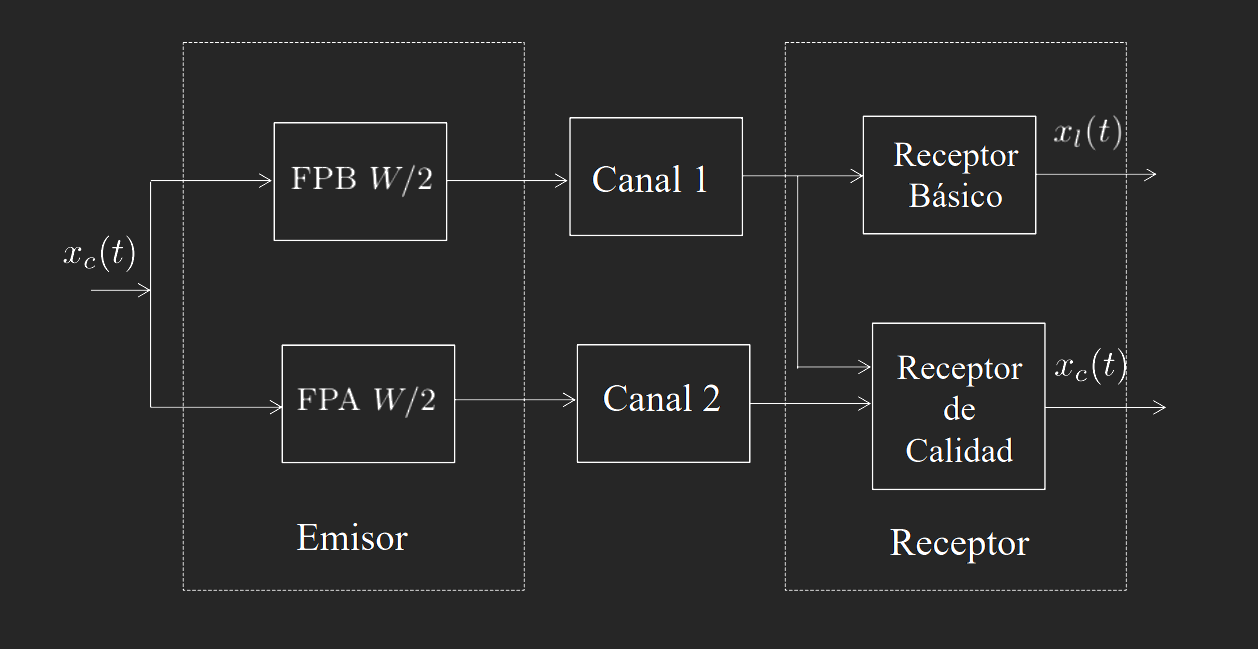
\includegraphics[width=0.8\textwidth]{fig1.jpg} 
    \caption{División de la señal original.}
    \label{fig:ejemplo}
\end{figure}

\begin{flushleft}
	Se decide implementar la idea utilizando transmisión y procesamiento digital, para lo cual se piensa utilizar el esquema de la figura 2 para el bloque transmisor. Este bloque recibe la señal original y devuelve al canal 1 la versión discreta paso-bajo de la misma, x1[n], y al canal 2 la parte paso-alto correspondiente a los detalles, x2[n]. El conversor C/D es un conversor ideal, y los filtros $H_0(e^{j \omega})$ y $H_1(e^{j \omega})$ son ideales, con una frecuencia de corte de 1/4 y ganancia 1, siendo paso bajo y paso alto respectivamente.
\end{flushleft}
\newpage

\begin{figure}[h!]
    \centering
    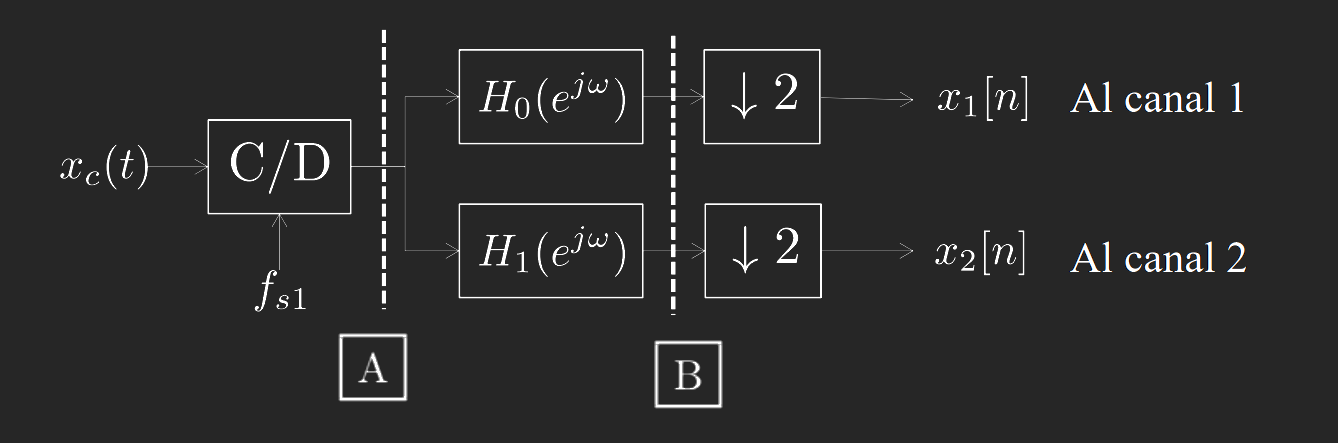
\includegraphics[width=0.5\textwidth]{fig2.jpg} 
    \caption{Sistema de procesado discreto para el transmisor.}
    \label{fig2:ejemplo2}
\end{figure}

\begin{figure}[h!]
    \centering
    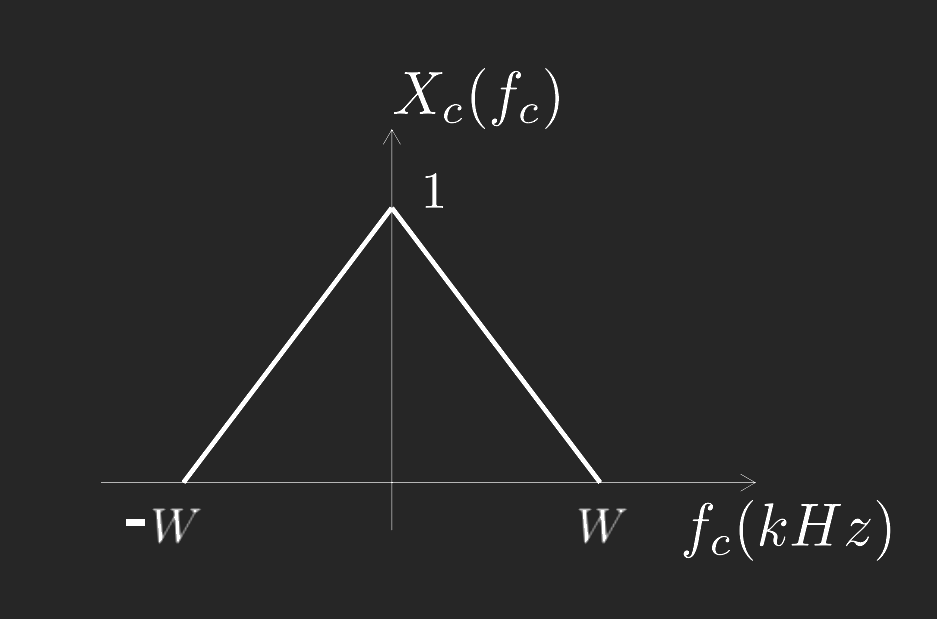
\includegraphics[width=0.5\textwidth]{fig3.jpg} 
    \caption{Espectro de la señal original.}
    \label{fig3:ejemplo3}
\end{figure}

\begin{flushleft}
    Suponiendo que el espectro de la señal original es el que se muestra en la figura 3, y que $f_{s1} = 8 \text{kHz}$
\end{flushleft}

\subsection{Calcular el ancho de banda máximo que puede tener la señal $x_{c}(t)$ para que no exista aliasing en el muestreo.}
Nyquist: $f_{s} \geq 2BW$
$$
W \leq 8 \text{kHz}
$$
\subsection{Dibujar el espectro de la señal discreta A.}

\begin{figure}[h!]
    \centering
    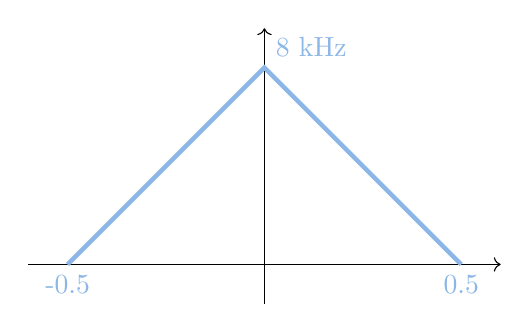
\begin{tikzpicture}
	    \draw[->, thin] (-3, 0) -- (3, 0);
	    \draw[->, thin] (0, -0.5) -- (0, 3);
	    \draw[c1, ultra thick] (-2.5, 0) node [below] {-0.5} -- (0, 2.5) node [above right] {8 kHz} -- (2.5, 0) node [below] {0.5};
    \end{tikzpicture}
\end{figure}
\subsection{Dibujar los espectros de la señal para ambos canales en el punto B}


\begin{figure}[h!]
    \centering
    \begin{minipage}{0.45\textwidth}
        \centering
        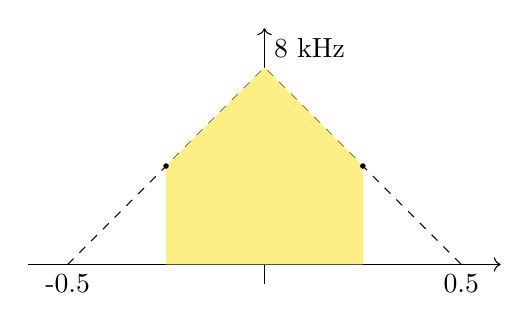
\begin{tikzpicture}[scale=0.5]
            \draw[->, thin] (-6, 0) -- (6, 0);
            \draw[->, thin] (0, -0.5) -- (0, 6);
            \draw[dashed] (-5, 0) coordinate(ini) node [below] {-0.5} -- (0, 5) coordinate(ver) node [above right] {8 kHz} -- (5, 0) coordinate(fin) node [below] {0.5};
            \coordinate (lowcut) at ($(ini)!.5!(ver)$);
            \coordinate (highcut) at ($(fin)!.5!(ver)$);
            \fill [c3] (lowcut |- 0,0) -- (lowcut) -- (ver) -- (highcut) -- (highcut |- 0,0);
            \fill (lowcut) circle (2 pt);
            \fill (highcut) circle (2 pt);
        \end{tikzpicture}
    \end{minipage}
    \begin{minipage}{0.45\textwidth}
        \centering
        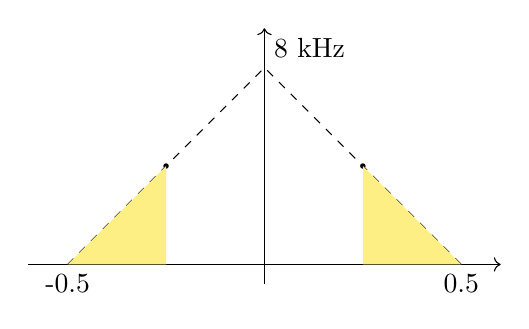
\begin{tikzpicture}[scale=0.5]
            \draw[->, thin] (-6, 0) -- (6, 0);
            \draw[->, thin] (0, -0.5) -- (0, 6);
            \draw[dashed] (-5, 0) coordinate(ini) node [below] {-0.5} -- (0, 5) coordinate(ver) node [above right] {8 kHz} -- (5, 0) coordinate(fin) node [below] {0.5};
            \coordinate (lowcut) at ($(ini)!.5!(ver)$);
            \coordinate (highcut) at ($(fin)!.5!(ver)$);
            \fill (lowcut) circle (2 pt);
            \fill (highcut) circle (2 pt);
            \fill [c3] (lowcut) -- (ini) -- (lowcut |- 0,0);
            \fill [c3] (highcut) -- (fin) -- (highcut |- 0,0);
        \end{tikzpicture}
    \end{minipage}%

\end{figure}
\subsection{Dibujar los espectros de las señales $x_{1}[n]$ y $x_{2}[n]$.}
\begin{figure}[h!]
    \centering
    \begin{minipage}{0.49\textwidth}
        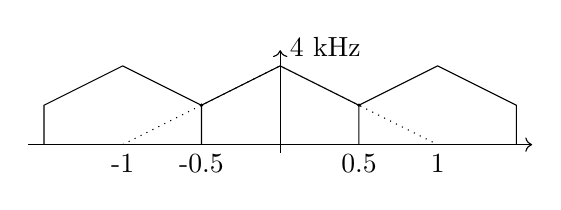
\begin{tikzpicture}[scale=0.2]
            \draw[->, thin] (-16, 0) -- (16, 0);
            \draw[->, thin] (0, -0.5) -- (0, 6);
            \draw[dotted] (-10, 0) coordinate(ini) node [below] {-1} -- (0, 5) coordinate(ver) node [above right] {4 kHz} -- (10, 0) coordinate(fin) node [below] {1};
            \coordinate (lowcut) at ($(ini)!.2!(ver)$);
            \coordinate (highcut) at ($(fin)!.2!(ver)$);
	    \coordinate (mid1) at ($(ini)!.5!(ver)$);
	    \coordinate (mid2) at ($(ver)!.5!(fin)$);
    \draw (mid1 |- 0,0) -- (mid1) circle (2 pt) -- (ver) -- (mid2) circle (2 pt) -- (mid2 |- 0,0);
    \draw (mid1) -- (-10, 0 |- ver) -- (-15, 0 |- mid1) -- (-15, 0);
    \draw (mid2) -- (10, 0 |- ver) -- (15, 0 |- mid1) -- (15, 0);
    \draw (5, 0) node [below] {0.5};
    \draw (-5, 0) node [below] {-0.5};
        \end{tikzpicture}
\end{minipage}%
    \begin{minipage}{0.49\textwidth}
        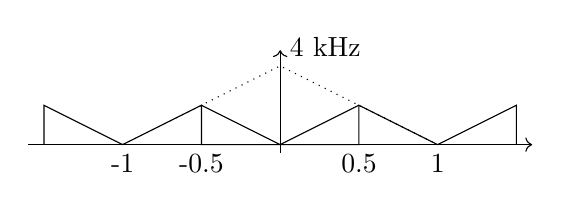
\begin{tikzpicture}[scale=0.2]
            \draw[->, thin] (-16, 0) -- (16, 0);
            \draw[->, thin] (0, -0.5) -- (0, 6);
            \draw[dotted] (-10, 0) coordinate(ini) node [below] {-1} -- (0, 5) coordinate(ver) node [above right] {4 kHz} -- (10, 0) coordinate(fin) node [below] {1};
            \coordinate (lowcut) at ($(ini)!.5!(ver)$);
            \coordinate (highcut) at ($(fin)!.5!(ver)$);
	    \draw (15, 0) -- (15, 0 |- highcut) -- (10, 0) -- (highcut) -- (5, 0) -- (-5, 0) -- (lowcut) -- (-10, 0) -- (-15, 0 |- lowcut) -- (-15, 0);
	    \draw (-5, 0 |- lowcut) -- (0, 0) -- (5, 0 |- lowcut);
    \draw (5, 0) node [below] {0.5};
    \draw (-5, 0) node [below] {-0.5};
        \end{tikzpicture}
\end{minipage}

\end{figure}
\subsection{Indicar el número de muestras por segundo que se envían a cada canal. Justifique su respuesta.}
Las muestras por segundo en ambos canales serán \( \frac{f_{s1}}{2} = 4000 \), ya que el número de muestras por segundo tras el muestreo era 8000 y la señal pasa por un diezmador por 2 antes de ser enviadas a los canales 1 y 2.


\end{document}
